% Chương 3

\chapter{KẾT QUẢ} % Tên của chương

\label{Chapter3} % Để trích dẫn chương này ở chỗ nào đó trong bài, hãy sử dụng lệnh \ref{Chapter3} 

%----------------------------------------------------------------------------------------

\section{Giao diện}

\begin{figure}[h!]
	\centering
	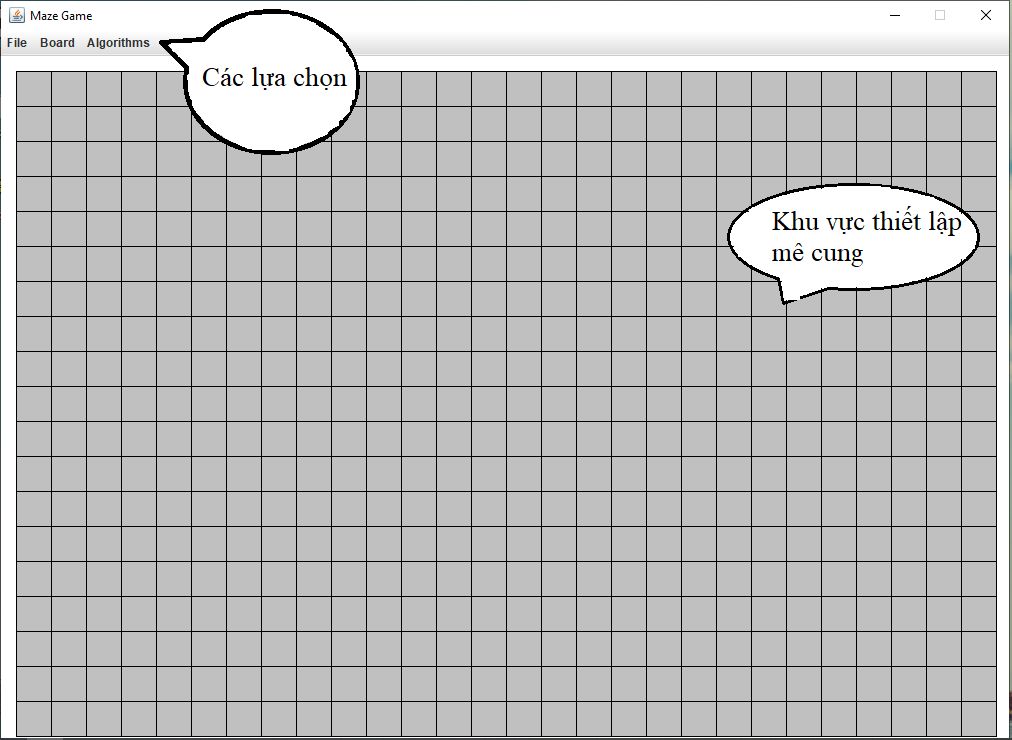
\includegraphics[width=0.8\textwidth]{
		Figures/figs/1.PNG
	}
	\caption[Giao diện game với phần tạo mê cung và các lựa chọn]{
		Giao diện game với phần tạo mê cung và các lựa chọn 
	}
	\label{fig:hinhe}
\end{figure}


\begin{figure}[h!]
	\centering
	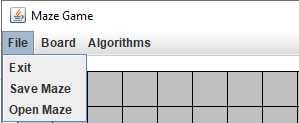
\includegraphics[width=0.8\textwidth]{
		Figures/figs/2.PNG
	}
	\caption[Chức năng lựa chọn File]{
		Chức năng lựa chọn File 
	}
	\label{fig:hinhf}
\end{figure}

Chức năng lựa chọn \textbf{File}:
\begin{itemize}
	\item Exit: Thoát khỏi trò chơi
	\item Save Maze: Lưu lại mê cung đã tạo vào máy
	\item Open Maze: Mở một mê cung đã có sẵn.
\end{itemize}

\begin{figure}[h!]
	\centering
	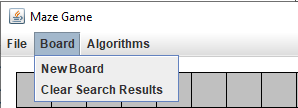
\includegraphics[width=0.8\textwidth]{
		Figures/figs/3.PNG
	}
	\caption[Chức năng lựa chọn Board:]{
		Chức năng lựa chọn Board: 
	}
	\label{fig:hinhg}
\end{figure}

Chức năng lựa chọn \textbf{Board}:
\begin{itemize}
	\item New Board: Tạo một giao diện trò chơi mới
	\item Clear Search Result: Xóa đường đi thuật toán đã tìm kiếm
\end{itemize}

\begin{figure}[h!]
	\centering
	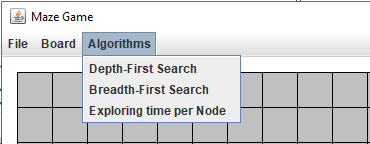
\includegraphics[width=0.8\textwidth]{
		Figures/figs/4.PNG 
	}
	\caption[Chức năng lựa chọn Algorithms]{
		Chức năng lựa chọn Algorithms 
	}
	\label{fig:hinhh}
\end{figure}

Chức năng lựa chọn \textbf{Algorithms}:
\begin{itemize}
	\item Depth-First Search: Sử dụng thuật toán DFS
	\item Breadth-First Search: Sử dụng thuật toán BFS
	\item Exploring time per Node: Cài đặt thời gian
\end{itemize}

\begin{figure}[h!]
	\centering
	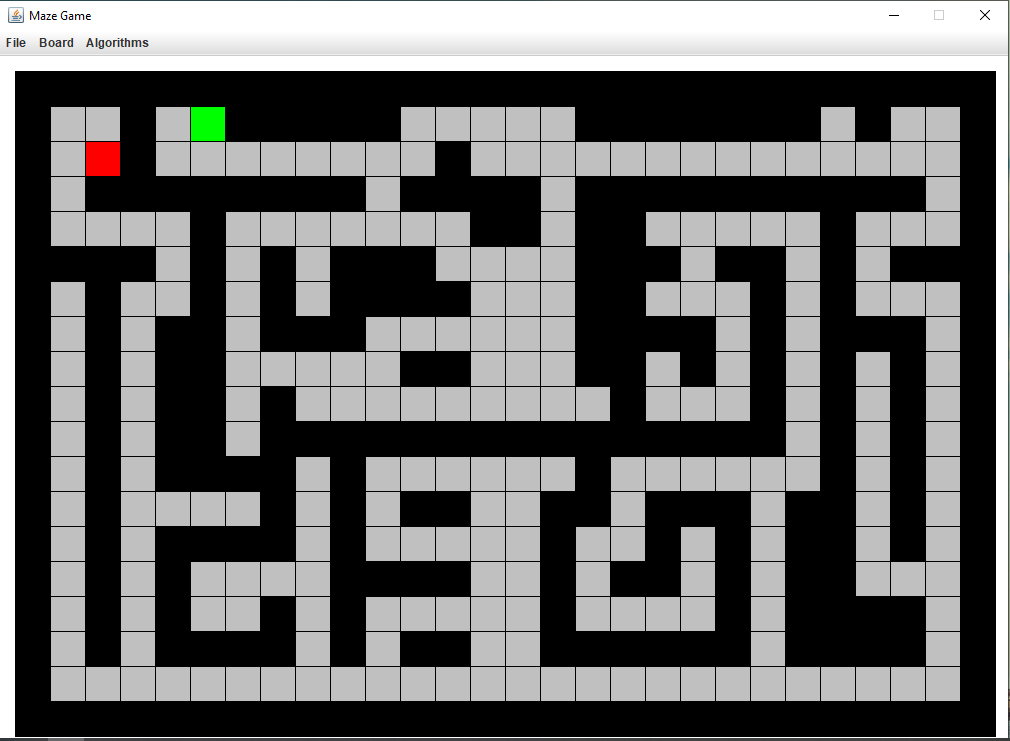
\includegraphics[width=0.7\textwidth]{
		Figures/figs/5.PNG
	}
	\caption[Giao diện mê cung đã được thiết lập với các thông tin]{
		Giao diện mê cung đã được thiết lập với các thông tin	 
	}
	\label{fig:hinhi}
\end{figure}

Giao diện mê cung đã được thiết lập với các thông tin:
\begin{itemize}
	\item Ô màu đen: Tường, chướng ngại vật không thể di chuyển qua được
	\item Ô màu xám: Vị trí có thể đi qua
	\item Ô màu đỏ: Vị trí đích
	\item Ô màu xanh: Vị trí bắt đầu
\end{itemize}

\newpage
\section{Kết quả}
\subsection{Thuật toán DFS}
\begin{figure}[h!]
	\centering
	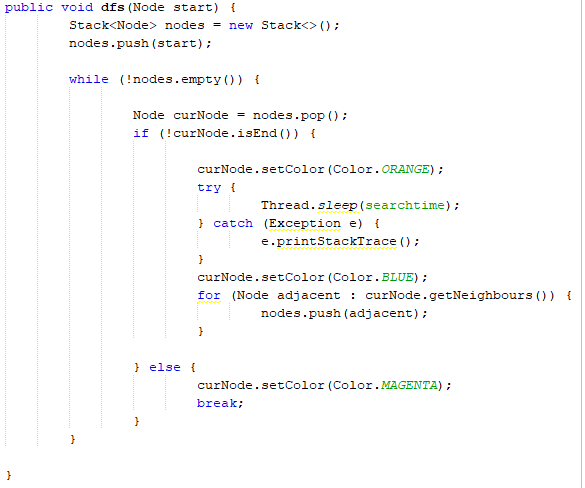
\includegraphics[width=0.8\textwidth]{
		Figures/figs/8.PNG
	}
	\caption[Thuật toán DFS tìm kiếm đường đi theo chiều sâu]{
		Thuật toán DFS tìm kiếm đường đi theo chiều sâu
	}
	\label{fig:hinhK}
\end{figure}

Trong đó:
\begin{enumerate}
	\item Tạo một đối tượng 'Stack<Node>' để lưu trữ các nút chưa được duyệt trong quá trình tìm kiếm.
	\item Đưa nút 'start' vào 'Stack' và bắt đầu vòng lặp while khi 'Stack' chưa rỗng.
	\item Lấy ra nút đầu tiên trong 'Stack' dùng 'pop()'
	\item Kiểm tra nếu nút hiện tại là nút đích ('isEnd()') thì đổi màu thành màu Magenta và dừng thuật toán.
	
	\item Nếu nút không phải đích, đổi màu thành màu cam và ngủ trong một khoảng thời gian (tùy chọn).
	\item Đổi màu của nút về màu xanh dương và thêm các nút kề vào 'Stack'.
	\item Lặp lại từ bước 3.
	\item Khi thuật toán kết thúc, đường đi từ nút bắt đầu đến nút đích sẽ được tô màu Magenta.
\end{enumerate}

\begin{figure}[h!]
	\centering
	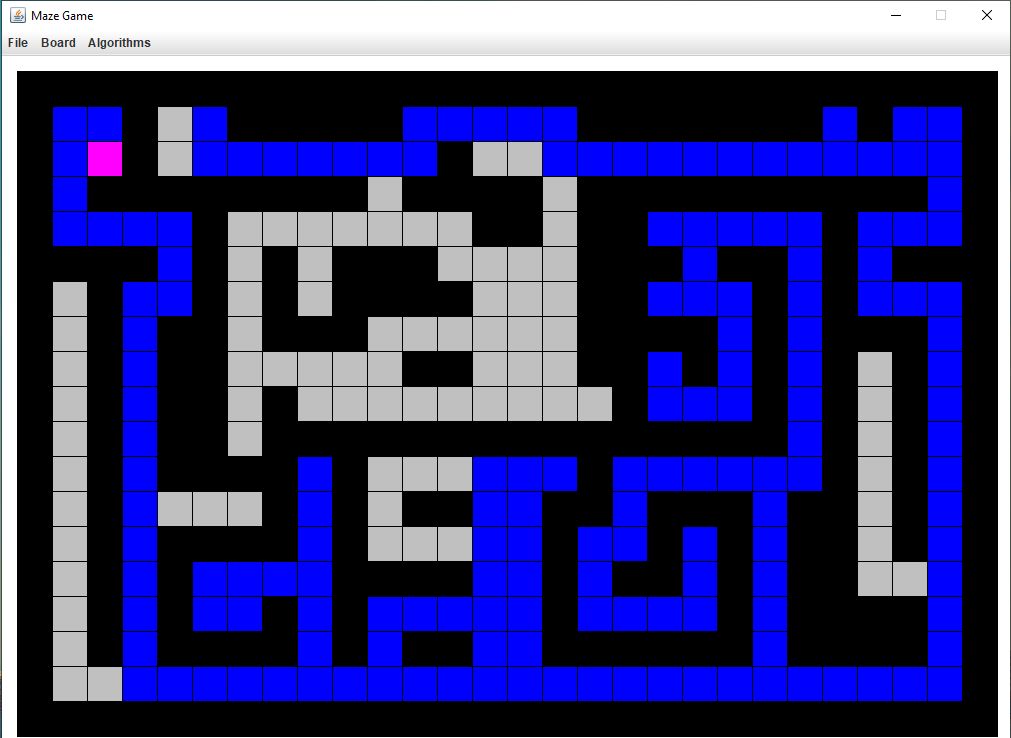
\includegraphics[width=0.8\textwidth]{
		Figures/figs/6.PNG
	}
	\caption[Kết quả tìm kiếm đường đi ma trận bằng thuật toán DFS]{
		Kết quả tìm kiếm đường đi ma trận bằng thuật toán DFS
	}
	\label{fig:hinhl}
\end{figure}

\newpage
\subsection{Thuật toán BFS}
\begin{figure}[h!]
	\centering
	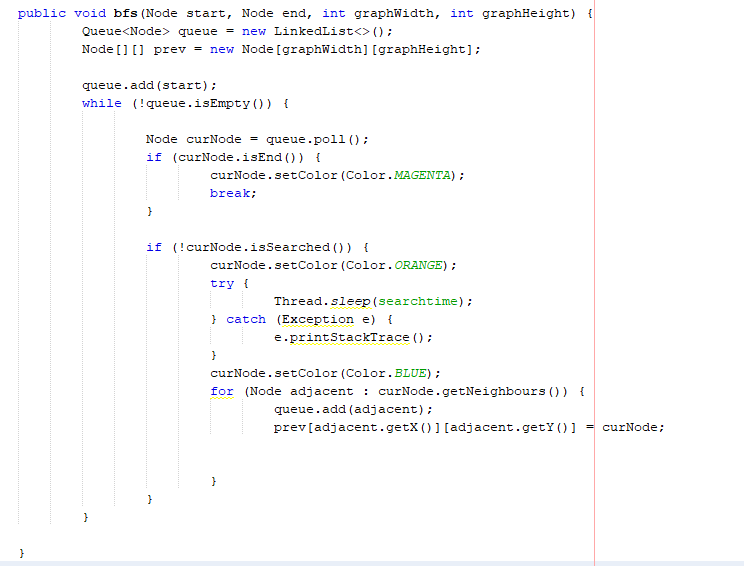
\includegraphics[width=0.8\textwidth]{
		Figures/figs/9.PNG
	}
	\caption[Thuật toán BFS tìm kiếm đường đi theo chiều rộng]{
		Thuật toán BFS tìm kiếm đường đi theo chiều rộng 
	}
	\label{fig:hinhm}
\end{figure}

Trong đó:
\begin{enumerate}
	\item Tạo một 'Queue<Node>' để lưu trữ các nút chưa được duyệt.
	\item Khởi tạo một mảng 2 chiều 'Node[][]' để lưu trữ nút đi trước của nút hiện tại.
	\item Thêm nút 'start' vào hàng đợi ('queue') và bắt đầu vòng lặp while khi hàng đợi chưa rỗng.
	\item Lấy nút đầu tiên ra khỏi hàng đợi dùng 'poll()'.
	\item Nếu nút là nút đích ('isEnd()'), thì đổi màu của nút thành Magenta, và kết thúc thuật toán.
	\item Nếu nút chưa được tìm kiếm, thì đổi màu thành Orange và ngủ một khoảng thời gian tùy chọn.
	\item Đổi màu của nút về màu Blue và thêm các nút kề của nó vào hàng đợi ('queue').
	\item Lưu trữ nút đóng vai trò là nút đi trước của nút hợp lệ trong mảng prev dựa trên vị trí hàng và cột của nút trong đồ thị.
	\item Lặp lại từ bước 4.
	\item Khi thuật toán kết thúc, tìm đường đi ngắn nhất từ nút 'start' đến nút 'end' sử dụng mảng 'prev' và sắp xếp các nút trên đường đi này thành màu Magenta.
\end{enumerate}

\begin{figure}[h!]
	\centering
	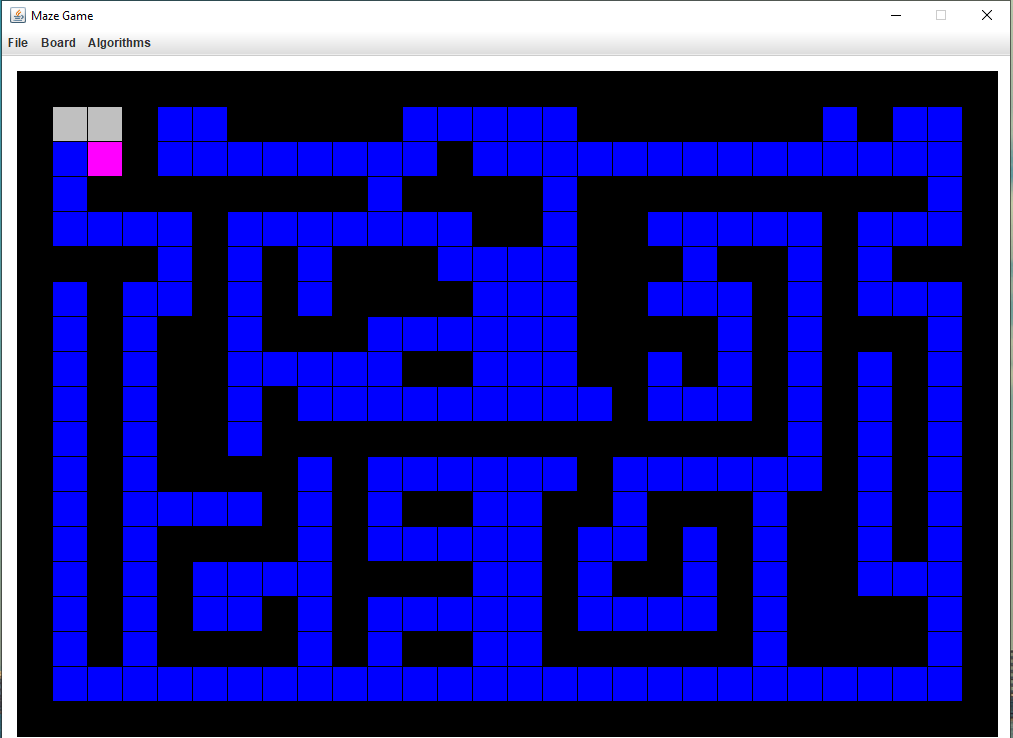
\includegraphics[width=0.6\textwidth]{
		Figures/figs/7.PNG
	}
	\caption[Kết quả tìm kiếm đường đi ma trận bằng thuật toán BFS]{
		Kết quả tìm kiếm đường đi ma trận bằng thuật toán BFS
	}
	\label{fig:hinhn}
\end{figure}


